\documentclass{article}

\usepackage[margin=20pt]{geometry}
\usepackage{graphics}
\graphicspath{{figures/}{../figures/}}

\usepackage{amsmath, amssymb, amsfonts}

\newcommand{\ie}{{\it i.e.~}}
\newcommand{\eg}{{\it e.g.~}}
\newcommand{\nb}{{\it n.b.~}}
\newcommand{\cfr}{{\it cfr.~}}
\newcommand{\viz}{{\it viz.~}}
\newcommand{\etc}{{\it etc.~}}
\newcommand{\sic}{{\it sic.~}}
\newcommand{\wrt}{{w.r.t.~}}

\usepackage{pgfplots}
\pgfplotsset{compat=1.18}

\usepackage{zx-calculus}
\usepackage{quantikz}
\usepackage{braket}
\usepackage{subcaption}

\tikzstyle{quantumR}=[red!75!black!50]
\tikzstyle{quantumB}=[blue!75!black!50]
\tikzstyle{quantumG}=[green!75!black!50]
\tikzstyle{quantumY}=[yellow!95!black!75]

\tikzstyle{data}=[circle, fill=black, text=white]
\tikzstyle{meas}=[circle, fill=white, draw=black, ultra thick]
\tikzstyle{stabilizer}=[draw=black]

\newcommand{\ttbf}{\ttfamily\fontseries{b}\selectfont}
\DeclareMathAlphabet{\mathpzc}{OT1}{pzc}{m}{it}

\title{TQEC --- Notes on T-state cultivation\footnote{Based on Austin Fowler's presentation of arXiv:2510.24615 and arXiv:2409.17595 at TQEC meeting on 2026/08/12.}}
\author{Seweryn Dynerowicz}
%\date{}

\newcommand{\Op}[1]{{\bf #1}}
\newcommand{\kett}[1]{\ket{\mbox{\tt #1}}}
\newcommand{\wn}{\wireoverride{n}}

\begin{document}
	\maketitle

	\section{Stage I --- Injection}
	
	The goal of the injection stage is to prepare a logical magic state\footnote{Note that the $\kett{0}_{\scriptscriptstyle L}$ and $\kett{1}_{\scriptscriptstyle L}$ are the logical states of the Steane Code, not the physical ones.} encoded with the Steane Code on 7 qubits.
	\begin{equation}
		\ket{\Op{T}}_{\scriptscriptstyle L} \quad=\quad
			\sqrt{\frac{1}{2}}\left(\vphantom{\sqrt{\frac{1}{2}}}
				\kett{0}_{\scriptscriptstyle L} + e^{i\pi/4}\kett{1}_{\scriptscriptstyle L}
			\right)
		\label{eq:magic-state}
	\end{equation}

	The injection stage is broken down into two main parts as shown on the figure below.
	\vspace{-1cm}

	\begin{figure}[h!]
		\centering
		\begin{quantikz}[row sep={between origins, 0.75cm}]
			& \gate[7,style={rounded corners=5pt}][3cm]{\textsc{Inject}}
			& \gate[7,style={rounded corners=5pt}][3cm]{\textsc{Syndrome}}
			& \gate[7,style={rounded corners=5pt, fill=black, inner ysep=-27.5pt}]{\rotatebox{90}{\color{white}\scshape Post-select}}
			& \\
			&&&& \\
			&&&& \\
			&&&& \\
			&&&& \\
			&&&& \\
			&&&&
		\end{quantikz}
		\vspace{-1cm}
		\caption{Overview of the injection stage in three parts.}	
	\end{figure}

	In the first part, an attempt is made to prepare a logical magic state using a modified Steane Code circuit where a phase of $e^{i\pi/4}$ is injected into a logical $\kett{+}_{\scriptscriptstyle L}$ state. \\

	Since we are working in a noisy environment, that attempt may fail and we wish to confirm whether the state that was prepared is indeed the one from Eq. (\ref{eq:magic-state}). The second part consists in performing a single round of syndrome measurement for the stabilizers of the Steane Code to determine whether the injection has successfully prepared a +1 eigenstate. A post-selection is performed based on the outcome to decide whether to discard the state and start a new attempt or proceed with the cultivation stage. The cultivation stage is where we verify that the correct phase has been injected and improve the code distance of the patch where that state is stored. \\

		% The syndrome measurement can only determine whether we have successfully prepared a logical $\kett{+}_{\scriptscriptstyle L}$. It is oblivious to the phase ?

	In the next subsections, we will go over the abstract circuitry behind those parts. The concrete circuits for the surface code array will be provided in the (TBD) appendix.

	\newpage

	\subsection{\mbox{\sc Inject} --- Modified Steane Code}

	In order to prepare a 7-qubits magic state, the following modified Steane Code circuit\footnote{Based on the circuit from Figure 6 in arXiv:2409.17595} is used where a $\Op{T}^\dagger$-gate\footnote{Or an $\Op{S}^\dagger$-gate to enable simulation of the resulting circuit that the non-Clifford \Op{T}-gate prevents} has been strategically placed to inject the $\frac{\pi}{4}$ phase onto the $\kett{1}_{\scriptscriptstyle L}$ component of the $\kett{+}_{\scriptscriptstyle L}$ state. In the following circuit, we assume a numbering of qubits $1$ through $7$ from top to bottom. 

	\begin{figure}[h!]
		\centering
		\begin{subfigure}[c]{0.32\textwidth}
			\centering
			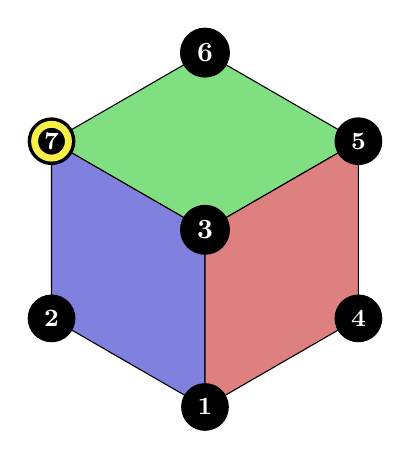
\begin{tikzpicture}
				\coordinate (O) at (0,0);
				\coordinate (A) at ( 30:2.25);
				\coordinate (B) at ( 90:2.25);
				\coordinate (C) at (150:2.25);
				\coordinate (D) at (210:2.25);
				\coordinate (E) at (270:2.25);
				\coordinate (F) at (330:2.25);

				\fill[quantumG, stabilizer] (O) -- (A) -- (B) -- (C) -- cycle;
				\fill[quantumB, stabilizer]  (O) -- (C) -- (D) -- (E) -- cycle;
				\fill[quantumR, stabilizer]  (O) -- (E) -- (F) -- (A) -- cycle;

				\node[data] at (E) {\small $\mathbf{1}$};
				\node[data] at (D) {\small $\mathbf{2}$};
				\node[data] at (O) {$\mathbf{3}$};
				\node[data] at (F) {\small $\mathbf{4}$};
				\node[data] at (A) {\small $\mathbf{5}$};
				\node[data] at (B) {$\mathbf{6}$};
				\node[data] at (C) {\small $\mathbf{7}$};
				\node[circle, draw=yellow!95!black!75, line width=2.5pt] at (C) {\phantom{.}};
			\end{tikzpicture}
		\end{subfigure}
		\begin{subfigure}[c]{0.62\textwidth}
			\centering
			\begin{quantikz}[row sep=0.6cm]
				\lstick{$\kett{+}$~} & \ctrl{1} &           & \ctrl{3}  &           &
				\slice{} &&&&&& \rstick[7]{~~$\ket{\Op{T}}_{\scriptscriptstyle L}$} \\
				\lstick{$\kett{0}$~} & \targ{}  & \targ{}   &\phantom{i}& \targ{}   &
				& \ctrl{5}  &&& \ctrl{5}  && \\
				\lstick{$\kett{+}$~} & \ctrl{1} & \ctrl{-1} &\phantom{i}&\phantom{i}& \ctrl{3}
				& \phantom{i}&&&\phantom{i}&& \\
				\lstick{$\kett{0}$~} & \targ{}  & \targ{}   & \targ{}   &\phantom{i}&\phantom{i}
				& \phantom{i}&&&\phantom{i}&& \\
				\lstick{$\kett{+}$~} & \ctrl{1} & \ctrl{-1} &           &\phantom{i}&\phantom{i}
				& \phantom{i}&&&\phantom{i}&& \\
				\lstick{$\kett{0}$~} & \targ{}  & \targ{}   &           &\phantom{i}& \targ{}
				& \phantom{i}&\ctrl{1}&&\phantom{i}& \ctrl{1} & \\[-0.2cm]
				\lstick{$\kett{+}$~} &          & \ctrl{-1} &           & \ctrl{-5} & 
				& \targ{}  & \targ{}  & \gate[style={fill=yellow!95!black!75}]{\Op{T}^{\dagger}} & \targ{} & \targ{} &
			\end{quantikz}
		\end{subfigure}
		\caption{Modified Steane Code with stabilizer diagram. Note that the abstract circuit can be performed in $8$ steps.}
	\end{figure}

	In the absence of errors, the seven qubits are in a logical state $\kett{+}_{\scriptscriptstyle L}$ once the red line is reached
	
	\begin{equation*}
		\kett{+}_{\scriptscriptstyle L} \quad=\quad
			\sqrt{\frac{1}{2}}\left(\vphantom{\sqrt{\frac{1}{2}}}
				\kett{0}_{\scriptscriptstyle L} + \kett{1}_{\scriptscriptstyle L}
			\right)
		\label{eq:logical-plus-state}
	\end{equation*}

	As pointed out by Austin, the first two CNOTs after the red line result in all the states of the logical $\kett{0}_{\scriptscriptstyle L}$ (resp. $\kett{1}_{\scriptscriptstyle L}$) having qubit $7$ set to $\kett{0}$ (resp. $\kett{1}$). Once the $e^{i\pi/4}$ phase has been injected by the $\Op{T}^{\dagger}$, the last two CNOTs change the value of qubit $7$ as to return the seven qubits in the state $\kett{+}_{\scriptscriptstyle L}$. See Figure (\ref{fig:injection-states}) for the detailed superpositions.

	\subsubsection{Proof of correctness}

	\paragraph{(TBD) Preparation of $\kett{+}_{\scriptscriptstyle L}$ } Sticking to our assumed numbering, the stabilizers propagate along the first five steps as follows

	\begin{equation*}
		\Op{X}_{1} \rightarrow \Op{X}_{124}
		\qquad
		\Op{X}_{3} \rightarrow \Op{X}_{2346}
		\qquad
		\Op{X}_{5} \rightarrow \Op{X}_{456}
		\qquad
		\Op{X}_{7} \rightarrow \Op{X}_{267}
		\qquad
		\Op{Z}_{2} \rightarrow \Op{Z}_{1237}
		\qquad
		\Op{Z}_{4} \rightarrow \Op{Z}_{1345}
		\qquad
		\Op{Z}_{6} \rightarrow \Op{Z}_{3567}
	\end{equation*}

	All those stabilizers commute with one another and we can derive the usual three 4-body X-stabilizers matching with the Z-stabilizers
	\begin{equation*}
		\Op{X}_{124}\Op{X}_{2346}\Op{X}_{267} = \Op{X}_{1237}
		\qquad
		\Op{X}_{124}\Op{X}_{2346}\Op{X}_{456} = \Op{X}_{1345}
		\qquad
		\Op{X}_{2346}\Op{X}_{456}\Op{X}_{267} = \Op{X}_{3567}
	\end{equation*}

%	The product of all the 4-body X-stabilizers tells us we have prepared the +1 eigenstate of logical $\Op{X}_{\scriptscriptstyle L}$
%	\begin{equation*}
%		\Op{X}_{124}\Op{X}_{2346}\Op{X}_{456}\Op{X}_{267} = \Op{X}_{1234567}
%	\end{equation*}

	\paragraph{(TBD) Injection of $e^{\pi/4}$ phase}

	\subsection{\mbox{\sc Syndrome} --- Detect preparation failure}

	\begin{figure}[h!]
		\centering
		\begin{quantikz}[row sep={between origins, 0.75cm}, column sep={between origins, 0.75cm}]
			\lstick{$q_1$} &&&\targ{}&&\ctrl{2}{}&& \\
			\lstick{$q_2$} &&\targ{}&\phantom{i}&\ctrl{1}{}&\phantom{i}&& \\
			\lstick{$\kett{+}$}
			& \ctrl{1} &\ctrl{-1}&\ctrl{-2}&\targ{}&\targ{}&\ctrl{1}& \meter{\scalebox{0.5}{\Op{X}}} \\
			\lstick{$\kett{0}$}
			& \targ{} &\ctrl{2}&\ctrl{1}&\targ{}&\targ{}&\targ{}& \meter{} \\
			\lstick{$q_3$} &&\phantom{i}&\targ{}&\phantom{i}&\ctrl{-1}&& \\
			\lstick{$q_7$} &&\targ{}&&\ctrl{-2	}&&&
		\end{quantikz}
		\caption{Syndrome extraction using superdense coding for stabilizer $1237$}
	\end{figure}


	\newpage

	\section{Stage II --- Cultivation}

	\begin{figure}[h!]
		\centering
		\begin{subfigure}[c]{0.35\textwidth}
			\centering
			\scalebox{1.0}{
				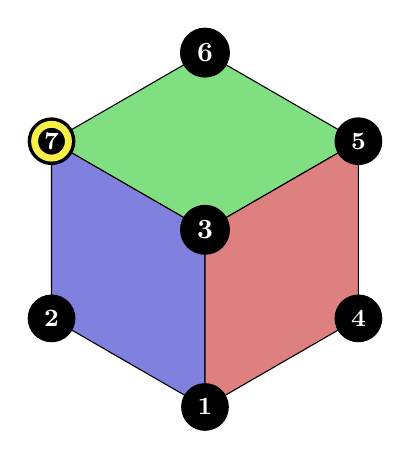
\begin{tikzpicture}
					\coordinate (O) at (0,0);
					\coordinate (A) at ( 30:2.25);
					\coordinate (B) at ( 90:2.25);
					\coordinate (C) at (150:2.25);
					\coordinate (D) at (210:2.25);
					\coordinate (E) at (270:2.25);
					\coordinate (F) at (330:2.25);
	
					\fill[quantumG, stabilizer] (O) -- (A) -- (B) -- (C) -- cycle;
					\fill[quantumB, stabilizer]  (O) -- (C) -- (D) -- (E) -- cycle;
					\fill[quantumR, stabilizer]  (O) -- (E) -- (F) -- (A) -- cycle;
	
					\node[data] at (E) {\small $\mathbf{1}$};
					\node[data] at (D) {\small $\mathbf{2}$};
					\node[data] at (O) {$\mathbf{3}$};
					\node[data] at (F) {\small $\mathbf{4}$};
					\node[data] at (A) {\small $\mathbf{5}$};
					\node[data] at (B) {$\mathbf{6}$};
					\node[data] at (C) {\small $\mathbf{7}$};
					\node[circle, draw=yellow!95!black!75, line width=2.5pt] at (C) {\phantom{.}};
				\end{tikzpicture}
			}
			\caption{Mapping of qubits onto the Steane Code. Qubit $7$ is the one on which the $\Op{T}^\dagger$ gate is applied in the injection stage.}
		\end{subfigure}
		\begin{subfigure}[c]{0.6\textwidth}
			\centering
			\begin{quantikz}[row sep={between origins, 0.75cm}]
				\lstick{$q_{6}$} & \gate[7,style={rounded corners=5pt}][1cm]{\Op{T}^\dagger}
				& \gate[7,style={rounded corners=5pt}][3cm]{\textsc{Cultivation}}
				& \gate[7,style={rounded corners=5pt}][1cm]{\Op{T}}
				& \\
				\lstick{$q_{7}$} &&&& \\
				\lstick{$q_{2}$} &&&& \\
				\lstick{$q_{3}$} &&&& \\
				\lstick{$q_{1}$} &&&& \\
				\lstick{$q_{5}$} &&&& \\
				\lstick{$q_{4}$} &&&&
			\end{quantikz}
			\caption{Overview of the cultivation stage in three parts.}	
		\end{subfigure}
	\end{figure}

	\begin{figure}[h!]
		\centering
		\begin{quantikz}[row sep={0.85cm, between origins}, column sep={0.3cm}]
			% Data qubit 6
			\lstick{$q_{6}$} & \gate{\Op{T}^\dagger} && \targ{} &\slice{}&&&&
			& &&&\slice{}&&\targ{} && \gate{\Op{T}} &
			\\
			% Ancilla 1
			&\wireoverride{n}& \midstick{$\kett{+}$}\wireoverride{n} & \ctrl{-1} && \targ{} &&&
			& &&&\targ{}&&\ctrl{-1} & \meter{\scalebox{0.5}{\Op{X}}} &&
			\\
			% Data qubit 7
			\lstick{$q_{7}$} & \gate{\Op{T}^\dagger} & &\targ{} && \ctrl{-1} &\targ{}&&
			& &&\targ{}&\ctrl{-1}&&\targ{}&&\gate{\Op{T}} &
			\\
			% Ancilla 2
			&\wireoverride{n}& \midstick{$\kett{+}$}\wireoverride{n} & \ctrl{-1} &&&\phantom{i}&&
			& &&\phantom{i}&&&\ctrl{-1}& \meter{\scalebox{0.5}{\Op{X}}} & \wn &
			\\
			% Data qubit 2
			\lstick{$q_{2}$} & \gate{\Op{T}^\dagger} & &\targ{} &&&\phantom{i}&&
			& &&\phantom{i}&&&\targ{}&&\gate{\Op{T}} &
			\\
			% Ancilla 3
			&\wireoverride{n}& \midstick{$\kett{+}$}\wireoverride{n} & \ctrl{-1} &&\targ{}&\phantom{i}&&
			& &&\phantom{i}&\targ{}&&\ctrl{-1}& \meter{\scalebox{0.5}{\Op{X}}} &&
			\\
			% Data qubit 3
			\lstick{$q_{3}$} & \gate{\Op{T}^\dagger} & &\targ{} &&\ctrl{-1}&\ctrl{-4}&\ctrl{3}& \meter{\scalebox{0.5}{\Op{X}}}
			& \wireoverride{}\midstick{$\kett{+}$} &\ctrl{3}&\ctrl{-4}&\ctrl{-1}&&\targ{}&& \gate{\Op{T}} &
			\\
			% Ancilla 4
			&\wireoverride{n}& \midstick{$\kett{+}$}\wireoverride{n} & \ctrl{-1} &&&&\phantom{i}&
			& &\phantom{i}&&&&\ctrl{-1}& \meter{\scalebox{0.5}{\Op{X}}} &&
			\\
			% Data qubit 1
			\lstick{$q_{1}$} & \gate{\Op{T}^\dagger} & &&\targ{}&&&\phantom{i}&
			& &&&&\targ{}&&&\gate{\Op{T}} &
			\\
			% Ancilla 5
			&\wireoverride{n}& \midstick{$\kett{+}$}\wireoverride{n} & \ctrl{1} &\ctrl{-1}&&\ctrl{2}&\targ{}&
			& &\targ{}&\ctrl{2}&&\ctrl{-1}&\ctrl{1}& \meter{\scalebox{0.5}{\Op{X}}} &&
			\\
			% Data qubit 5
			\lstick{$q_{5}$} & \gate{\Op{T}^\dagger} & &\targ{} &&&\phantom{i}&&
			& &&\phantom{i}&&&\targ{}&&\gate{\Op{T}} &
			\\
			% Ancilla 6
			&\wireoverride{n}& \midstick{$\kett{+}$}\wireoverride{n} & \ctrl{1} &&&\targ{}&&
			& &&\targ{}&&&\ctrl{1}& \meter{\scalebox{0.5}{\Op{X}}} &&
			\\
			% Data qubit 4
			\lstick{$q_{4}$} & \gate{\Op{T}^\dagger} & &\targ{} &&&&&
			& &&&&&\targ{}&&\gate{\Op{T}} &
		\end{quantikz}
		\caption{Highlight on the central part of the cultivation. Note that the qubits have been re-organised for a more readable circuit.}
	\end{figure}

	\newpage

	\section{Stage III --- Expansion}

	\newpage

	\appendix

	\section{Injection stage --- Extra diagrams}

	\begin{figure}[h!]
		\centering
		\scalebox{0.9}{
		\begin{quantikz}[row sep=0.6cm]
			\lstick{$\kett{+}$~} & \ctrl{1} &           & \ctrl{3}  &           &
			\slice{} & \midstick[7]{~~$\begin{aligned}
				  \kett{0000000} &+ \kett{1111111} \\
				+ \kett{1110001} &+ \kett{0001110} \\
				+ \kett{1011100} &+ \kett{0100011} \\ 
				+ \kett{0010111} &+ \kett{1101000} \\ 
				+ \kett{0101101} &+ \kett{1010010} \\
				+ \kett{1100110} &+ \kett{0011001} \\
				+ \kett{1001011} &+ \kett{0110100} \\ 
				+ \kett{0111010} &+ \kett{1000101} \\ 
			\end{aligned}$~~}
			&&& \midstick[7]{~~$\begin{aligned}
				  \kett{0000000} &+ \kett{1111111} \\
				+ \kett{1110000} &+ \kett{0001111} \\
				+ \kett{1011100} &+ \kett{0100011} \\ 
				+ \kett{0010110} &+ \kett{1101001} \\ 
				+ \kett{0101100} &+ \kett{1010011} \\
				+ \kett{1100110} &+ \kett{0011001} \\
				+ \kett{1001010} &+ \kett{0110101} \\ 
				+ \kett{0111010} &+ \kett{1000101} \\ 
			\end{aligned}$~~}
			&&&& \rstick[7]{~~$\ket{\Op{T}}_{\scriptscriptstyle L}$} \\
			\lstick{$\kett{0}$~} & \targ{}  & \targ{}   &\phantom{i}& \targ{}   &
			&&          & \ctrl{5}  &&& \ctrl{5}  && \\
			\lstick{$\kett{+}$~} & \ctrl{1} & \ctrl{-1} &\phantom{i}&\phantom{i}& \ctrl{3}
			&&          &\phantom{i}&&&\phantom{i}&& \\
			\lstick{$\kett{0}$~} & \targ{}  & \targ{}   & \targ{}   &\phantom{i}&\phantom{i}
			&&          &\phantom{i}&&&\phantom{i}&& \\
			\lstick{$\kett{+}$~} & \ctrl{1} & \ctrl{-1} &           &\phantom{i}&\phantom{i}
			&&          &\phantom{i}&&&\phantom{i}&& \\
			\lstick{$\kett{0}$~} & \targ{}  & \targ{}   &           &\phantom{i}& \targ{}
			&& \ctrl{1} &\phantom{i}&&&\phantom{i}& \ctrl{1} & \\[-0.2cm]
			\lstick{$\kett{+}$~} &          & \ctrl{-1} &           & \ctrl{-5} & 
			&& \targ{}  & \targ{}  && \gate{\Op{T}^{\dagger}} & \targ{} & \targ{} &
		\end{quantikz}
		}
		\caption{Modified Steane Code with intermediate states (normalisation factor omitted). The basis states corresponding to the $\kett{0}_{\scriptscriptstyle L}$ (resp. $\kett{1}_{\scriptscriptstyle L}$) are aligned in the left (resp. right) column. Note that the 7-th qubit has a value of $\kett{0}$ (resp. $\kett{1}$) in all the components coming from $\kett{0}_{\scriptscriptstyle L}$ (resp. $\kett{1}_{\scriptscriptstyle L}$) before the $\Op{T}^{\dagger}$-gate is applied.}
		\label{fig:injection-states}
	\end{figure}

	\newpage

	\section{Configurations for teleportation}

	\begin{figure}[h!]
		\centering
		\begin{subfigure}[b]{0.95\textwidth}
			\centering
			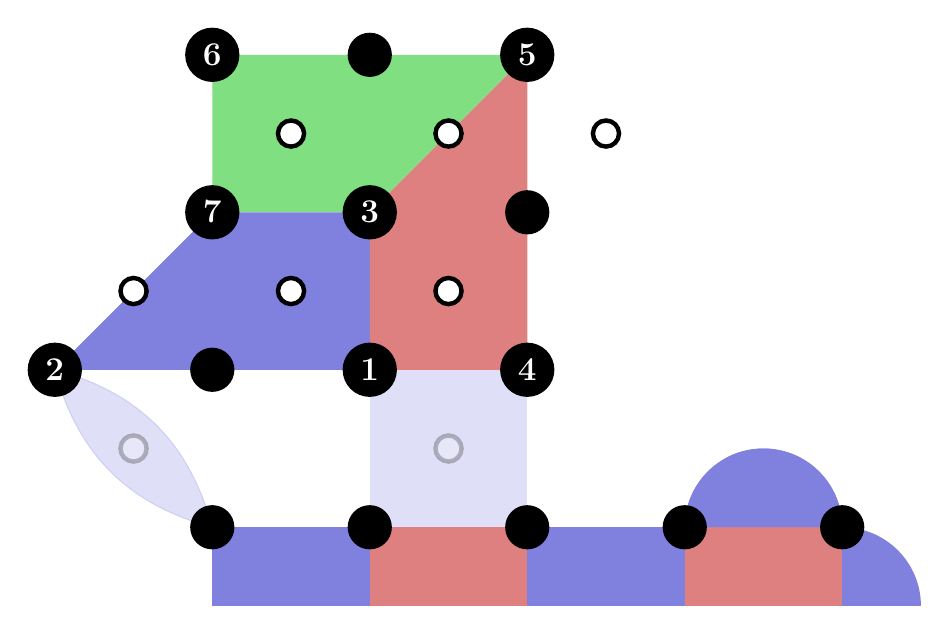
\begin{tikzpicture}
				% Plaquettes of the Steane Code
				\fill[quantumG] (0, 0) -- (4, 0) -- (2,-2) -- (0, -2);
				\fill[quantumB] (0,-2) -- (-2, -4) -- (2, -4) -- (2, -2);
				\fill[quantumR] (2,-2) -- (2, -4) -- (4, -4) -- (4, 0);
	
				% Plaquettes of the Surface Code
				\fill[quantumB] (0,-6) -- (2, -6) -- (2, -7) -- (0, -7);
				\fill[quantumB] (4,-6) -- (6, -6) -- (6, -7) -- (4, -7);
				\fill[quantumR] (2,-6) -- (4, -6) -- (4, -7) -- (2, -7);
				\fill[quantumR] (6,-6) -- (8, -6) -- (8, -7) -- (6, -7);
	
				\fill[quantumB] (6, -6) arc[start angle=180, end angle=0, radius=1.0]
					-- (8, -6) -- cycle;
				\fill[quantumB] (8, -6) arc[start angle=90, end angle=0, radius=1.0]
					-- (8, -7) -- cycle;
				\fill[quantumB] (6, -6) arc[start angle=180, end angle=0, radius=1.0]
					-- (8, -6) -- cycle;
	
				\fill[quantumB, opacity=0.25] (2,-4) -- (4, -4) -- (4, -6) -- (2, -6);
				\filldraw[quantumB, opacity=0.25] (-2,-4) to[bend left=30] (0,-6) to[bend left=30] (-2,-4);
	
	
				\node[data] at (2, 0) {\phantom{o}};
				\node[data] at (4,-2) {\phantom{o}};
				\node[data] at (0,-4) {\phantom{o}};
	
				\node[data] at (2,-4) {\large $\mathbf{1}$};
				\node[data] at (-2,-4) {\large $\mathbf{2}$};
				\node[data] at (2,-2) {\large $\mathbf{3}$};
				\node[data] at (4,-4) {\large $\mathbf{4}$};
				\node[data] at (4, 0) {\large $\mathbf{5}$};
				\node[data] at (0, 0) {\large $\mathbf{6}$};
				\node[data] at (0,-2) {\large $\mathbf{7}$};	
	
				\foreach \x in {1, 3, 5}{ \node[meas] at (\x,-1) {}; }
				\foreach \x in {-1, 1, 3}{ \node[meas] at (\x,-3) {}; }
				\foreach \x in {-1, 3}{ \node[meas, opacity=0.25] at (\x,-5) {}; }
	
				\foreach \x in {0, 2, 4, 6, 8}{ \node[data] at (\x, -6) {\phantom{o}}; }
			\end{tikzpicture}
			\caption{Modified Steane Code overlaid on the surface code array. Data qubits are identified as black circles. Measurement qubits are shown as white circles. The extra qubits (6 syndrome and 3 data) can be used to perform the superdense code cycle and the cultivation stage. The surface code onto which the magic state will be teleported is partially shown below for reference.}
		\end{subfigure}
		\vspace{0.5cm}
		\begin{subfigure}[b]{0.45\textwidth}
			\centering
			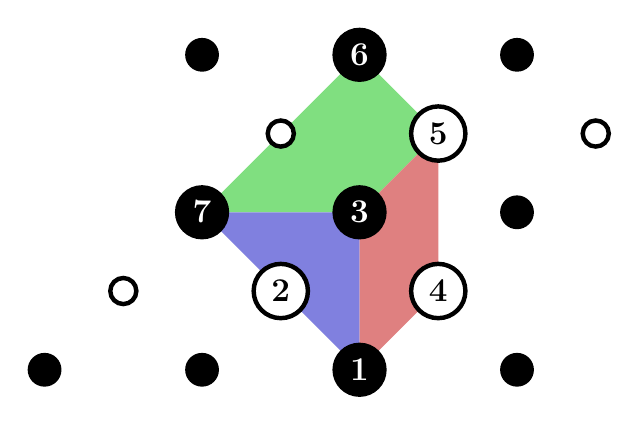
\begin{tikzpicture}
				% Plaquettes of the Steane Code
				\fill[quantumG] (2, 0) -- (3,-1) -- (2,-2) -- (0, -2);
				\fill[quantumB] (0,-2) -- (2, -4) -- (2, -2);
				\fill[quantumR] (2,-2) -- (3, -1) -- (3, -3) -- (2,-4);

				\node[data] at ( 2, 0) {\phantom{.}};
				\node[data] at ( 4,-2) {\phantom{.}};
				\node[data] at ( 0,-4) {\phantom{.}};
				\node[data] at (-2,-4) {\phantom{.}};

				\node[data] at (2,-4) {\large $\mathbf{1}$};
				\node[meas] at (1,-3) {\large $\mathbf{2}$};
				\node[data] at (2,-2) {\large $\mathbf{3}$};
				\node[meas] at (3,-3) {\large $\mathbf{4}$};
				\node[meas] at (3,-1) {\large $\mathbf{5}$};
				\node[data] at (2, 0) {\large $\mathbf{6}$};
				\node[data] at (0,-2) {\large $\mathbf{7}$};	

				\node[data] at ( 0, 0) {\phantom{.}};
				\node[data] at ( 4, 0) {\phantom{.}};
				\node[data] at ( 4,-4) {\phantom{.}};

				\foreach \x in {1, 5}{ \node[meas] at (\x,-1) {}; }
				\node[meas] at (-1,-3) {};
			\end{tikzpicture}
			\caption{Initial locations of the $7$ qubits for the Steane Code}
		\end{subfigure}
		\begin{subfigure}[b]{0.45\textwidth}
			\centering
			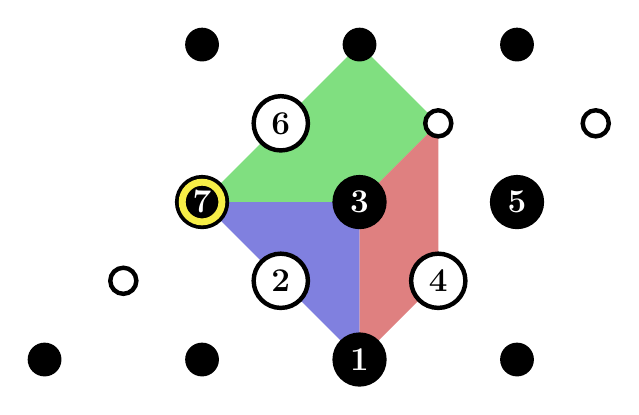
\begin{tikzpicture}
				% Plaquettes of the Steane Code
				\fill[quantumG] (2, 0) -- (3,-1) -- (2,-2) -- (0, -2);
				\fill[quantumB] (0,-2) -- (2, -4) -- (2, -2);
				\fill[quantumR] (2,-2) -- (3, -1) -- (3, -3) -- (2,-4);

				\node[data] at ( 2, 0) {\phantom{.}};
				\node[data] at ( 4,-2) {\phantom{.}};
				\node[data] at ( 0,-4) {\phantom{.}};
				\node[data] at (-2,-4) {\phantom{.}};

				\node[data] at (2,-4) {\large $\mathbf{1}$};
				\node[meas] at (1,-3) {\large $\mathbf{2}$};
				\node[data] at (2,-2) {\large $\mathbf{3}$};
				\node[meas] at (3,-3) {\large $\mathbf{4}$};
				\node[data] at (4,-2) {\large $\mathbf{5}$};
				\node[meas] at (1,-1) {\large $\mathbf{6}$};
				\node[data] at (0,-2) {\large $\mathbf{7}$};	
				\node[circle, draw=yellow!95!black!75, line width=2.5pt] at (0,-2) {\scalebox{0.75}{\phantom{o}}};

				\node[data] at ( 0, 0) {\phantom{.}};
				\node[data] at ( 4, 0) {\phantom{.}};
				\node[data] at ( 4,-4) {\phantom{.}};

				\foreach \x in {3, 5}{ \node[meas] at (\x,-1) {}; }
				\node[meas] at (-1,-3) {};
			\end{tikzpicture}
			\caption{Locations of the $7$ qubits when the $\Op{T}^\dagger$ gate is applied}
		\end{subfigure}
	\end{figure}

	\begin{figure}[h!]
		\centering
		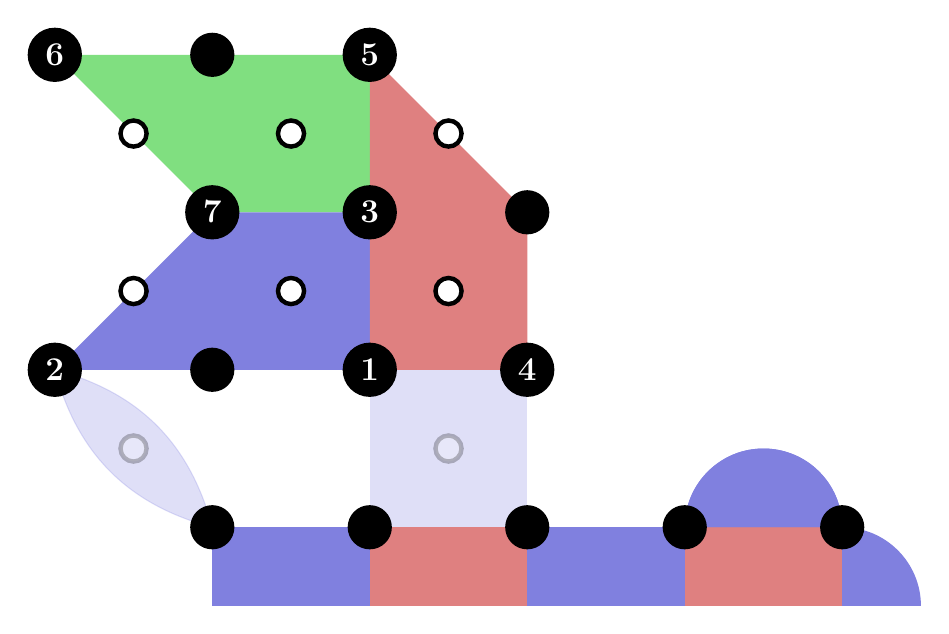
\begin{tikzpicture}
			% Plaquettes of the Steane Code
			\fill[quantumG] (-2, 0) -- ( 2, 0) -- ( 2,-2) -- ( 0,-2);
			\fill[quantumB]  ( 0,-2) -- (-2,-4) -- ( 2,-4) -- ( 2,-2);
			\fill[quantumR]   ( 2, 0) -- ( 4,-2) -- ( 4,-4) -- ( 2,-4);

			% Plaquettes of the Surface Code
			\fill[quantumB] (0,-6) -- (2, -6) -- (2, -7) -- (0, -7);
			\fill[quantumB] (4,-6) -- (6, -6) -- (6, -7) -- (4, -7);
			\fill[quantumR] (2,-6) -- (4, -6) -- (4, -7) -- (2, -7);
			\fill[quantumR] (6,-6) -- (8, -6) -- (8, -7) -- (6, -7);

			\fill[quantumB] (6, -6) arc[start angle=180, end angle=0, radius=1.0]
				-- (8, -6) -- cycle;
			\fill[quantumB] (8, -6) arc[start angle=90, end angle=0, radius=1.0]
				-- (8, -7) -- cycle;
			\fill[quantumB] (6, -6) arc[start angle=180, end angle=0, radius=1.0]
				-- (8, -6) -- cycle;

			\fill[quantumB, opacity=0.25] (2,-4) -- (4, -4) -- (4, -6) -- (2, -6);
			\filldraw[quantumB, opacity=0.25] (-2,-4) to[bend left=30] (0,-6) to[bend left=30] (-2,-4);


			\node[data] at ( 0, 0) {\phantom{o}};
			\node[data] at ( 4,-2) {\phantom{o}};
			\node[data] at ( 0,-4) {\phantom{o}};

			\node[data] at ( 2,-4) {\large $\mathbf{1}$};
			\node[data] at (-2,-4) {\large $\mathbf{2}$};
			\node[data] at ( 2,-2) {\large $\mathbf{3}$};
			\node[data] at ( 4,-4) {\large $\mathbf{4}$};
			\node[data] at ( 2, 0) {\large $\mathbf{5}$};
			\node[data] at (-2, 0) {\large $\mathbf{6}$};
			\node[data] at ( 0,-2) {\large $\mathbf{7}$};	

			\foreach \x in {-1, 1, 3}{
				\foreach \y in {-3, -1}{
					\node[meas] at (\x,\y) {};
				}
			}
			\foreach \x in {-1, 3}{ \node[meas, opacity=0.25] at (\x,-5) {}; }

			\foreach \x in {0, 2, 4, 6, 8}{ \node[data] at (\x, -6) {\phantom{o}}; }
		\end{tikzpicture}
		\caption{(Alternative) Modified Steane Code overlaid on the surface code array. Data qubits are identified as black circles. Measurement qubits are shown as white circles. The extra qubits (6 syndrome and 3 data) can be used to perform the superdense code cycle and the cultivation stage. The surface code onto which the magic state will be teleported is partially shown below for reference.}
	\end{figure}
\end{document}
